%%%%%%%% ICML 2019 EXAMPLE LATEX SUBMISSION FILE %%%%%%%%%%%%%%%%%

\documentclass{article}

% Recommended, but optional, packages for figures and better typesetting:
\usepackage{microtype}
\usepackage{graphicx}
\usepackage{subfigure}
\usepackage{booktabs} % for professional tables
\usepackage{graphicx}

% hyperref makes hyperlinks in the resulting PDF.
% If your build breaks (sometimes temporarily if a hyperlink spans a page)
% please comment out the following usepackage line and replace
% \usepackage{icml2019} with \usepackage[nohyperref]{icml2019} above.
\usepackage{hyperref}

% Attempt to make hyperref and algorithmic work together better:
\newcommand{\theHalgorithm}{\arabic{algorithm}}

% Use the following line for the initial blind version submitted for review:
%\usepackage{icml2019}

% If accepted, instead use the following line for the camera-ready submission:
\usepackage[accepted]{icml2019}

% The \icmltitle you define below is probably too long as a header.
% Therefore, a short form for the running title is supplied here:
\icmltitlerunning{COSE474-2024F: Final Project Proposal}

\begin{document}

\twocolumn[
\icmltitle{COSE474-2024F: Final Project Proposal \\
           ``Harry Potter Dialogue Generation using LoRA and Prompt Tuning''}

% It is OKAY to include author information, even for blind
% submissions: the style file will automatically remove it for you
% unless you've provided the [accepted] option to the icml2019
% package.

% List of affiliations: The first argument should be a (short)
% identifier you will use later to specify author affiliations
% Academic affiliations should list Department, University, City, Region, Country
% Industry affiliations should list Company, City, Region, Country

% You can specify symbols, otherwise they are numbered in order.
% Ideally, you should not use this facility. Affiliations will be numbered
% in order of appearance and this is the preferred way.
\icmlsetsymbol{equal}{*}

\begin{icmlauthorlist}
\icmlauthor{2021170964 Kyoungbin Park}{}
\end{icmlauthorlist}
%\icmlaffiliation{ku}{Department of Computer Science \& Engineering, Korea University, Seoul, Korea}


%\icmlcorrespondingauthor{the}{myemail@korea.ac.kr}
%\icmlcorrespondingauthor{Eee Pppp}{ep@eden.co.uk}

% You may provide any keywords that you
% find helpful for describing your paper; these are used to populate
% the "keywords" metadata in the PDF but will not be shown in the document
\icmlkeywords{Machine Learning, ICML, Deep Learning, NLP, LLM, Mistral, Fine Tuning, Prompt Tuning}

\vskip 0.3in
]

% this must go after the closing bracket ] following \twocolumn[ ...

% This command actually creates the footnote in the first column
% listing the affiliations and the copyright notice.
% The command takes one argument, which is text to display at the start of the footnote.
% The \icmlEqualContribution command is standard text for equal contribution.
% Remove it (just {}) if you do not need this facility.

%\printAffiliationsAndNotice{}  % leave blank if no need to mention equal contribution
%\printAffiliationsAndNotice{\icmlEqualContribution} % otherwise use the standard text.

%\begin{abstract}
%This document provides a basic paper template and submission guidelines.
%Abstracts must be a single paragraph, ideally between 4--6 sentences long.
%Gross violations will trigger corrections at the camera-ready phase.
%\end{abstract}



\section{Introduction}
The remarkable success of subculture games like Genshin Impact, Star Rail, Zenless Zone Zero, and Wuthering Waves demonstrates the substantial market demand for this genre. Among the numerous subculture games available, titles from HoYoverse and Kuro Games consistently achieve exceptional revenue primarily due to three key factors: distinct character personalities, compelling storylines, and immersive dialogue interactions with these characters.
However, current dialogue systems in subculture games face significant limitations due to their predetermined nature. This creates two major challenges:
\begin{itemize}
\item \textbf{Limited Player Agency}: Players often must select from predetermined responses, sometimes forcing them into dialogue choices that don't align with their preferred interaction style.
\item \textbf{Resource-Intensive Content Creation}: Companies must pre-generate all dialogue content before release, requiring substantial time and financial investment. This prevents players from engaging in new conversations with characters they've grown attached to unless the company releases updates.
\end{itemize}
These limitations lead to a gradual decline in character engagement over time, as companies lack incentive to continuously produce new content for existing characters. This project explores the potential of replacing static dialogue systems with LLM-powered conversations that maintain the richness and character-specific nuances of hand-crafted dialogue while offering dynamic, real-time interactions.



\graphicspath{ {./images/} }

\begin{figure*}[t]  % t는 top을 의미
    \centering
    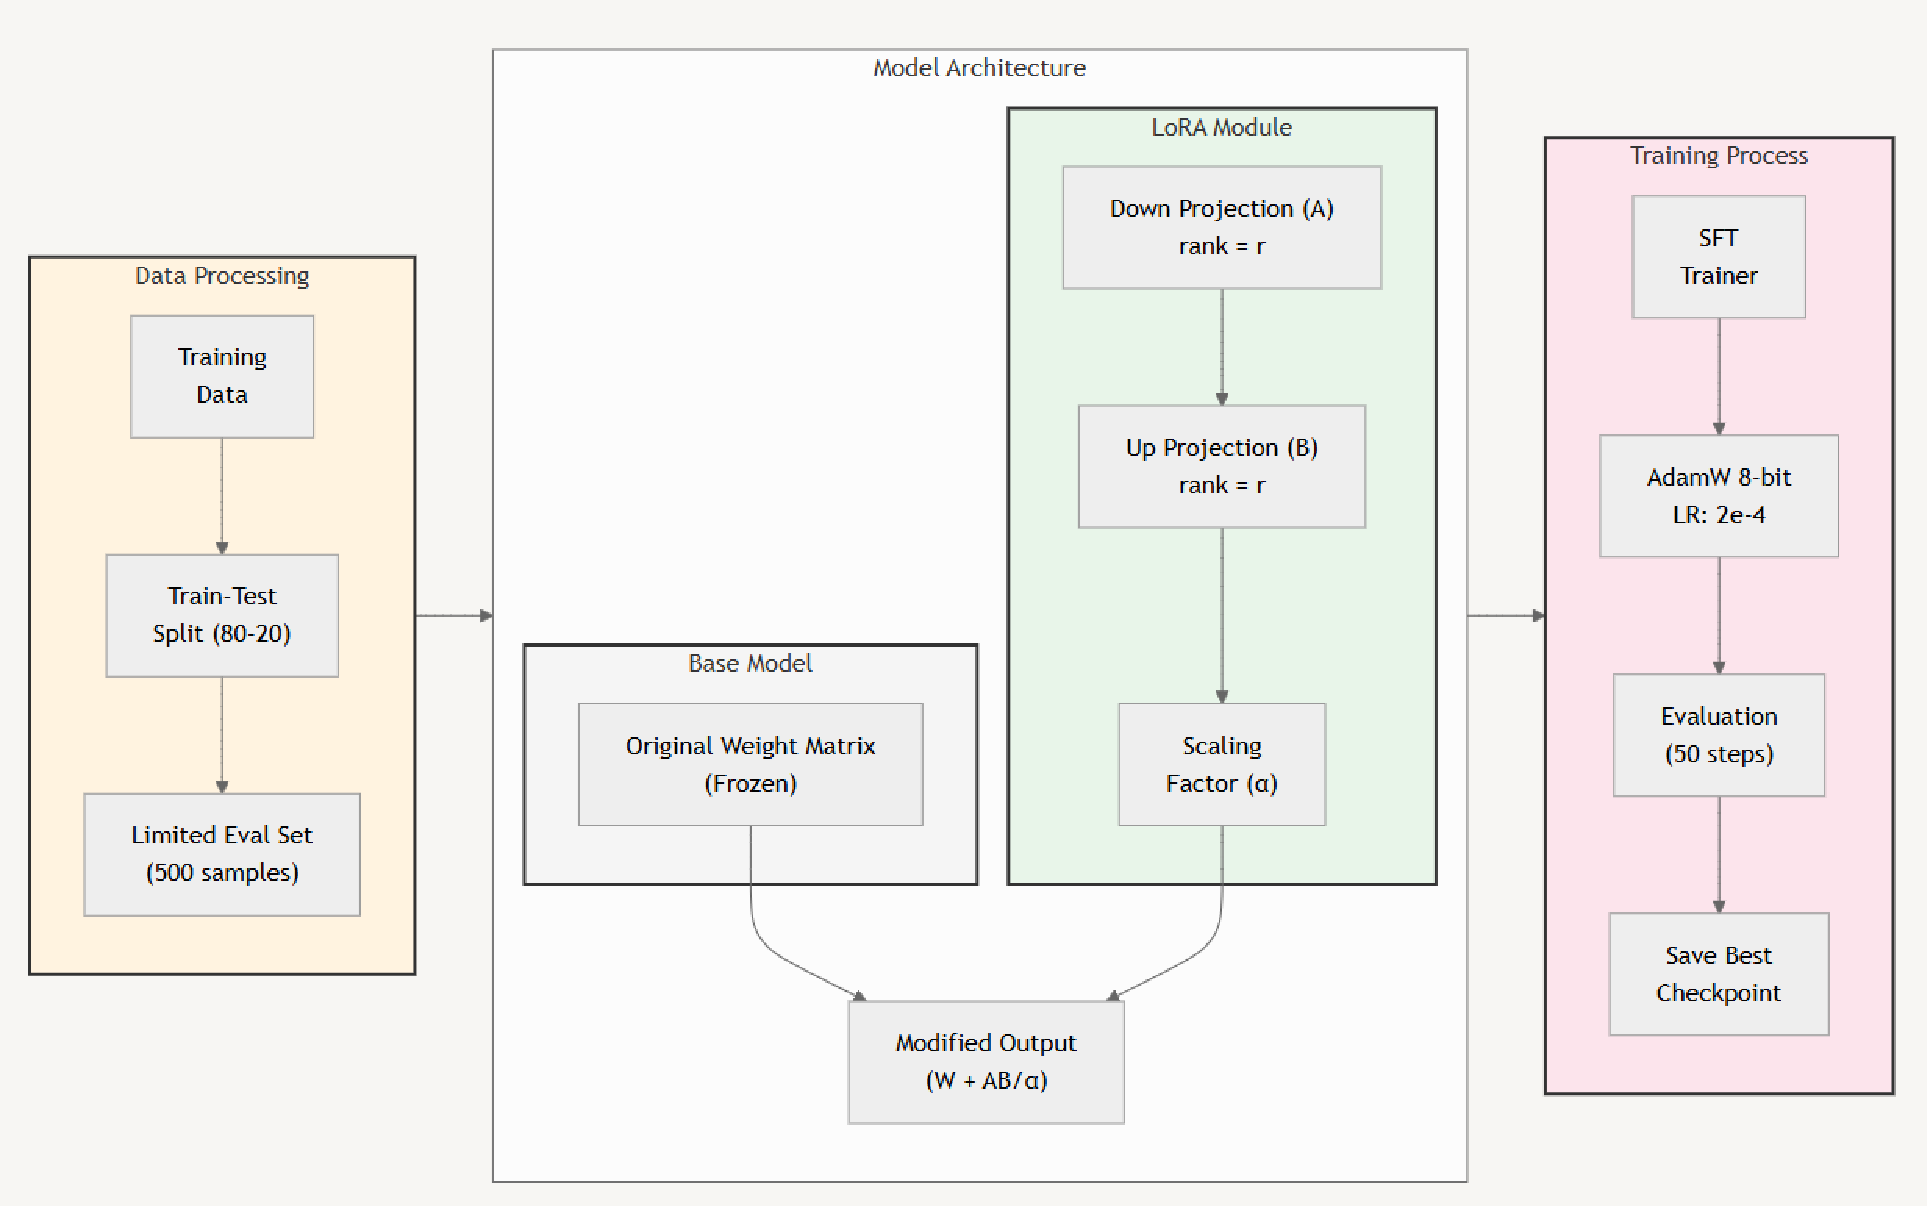
\includegraphics[width=0.8\textwidth]{./lora_model}
    \caption{LoRA}
    \label{fig:lora-model}
\end{figure*}

\begin{figure*}[t]
    \centering
    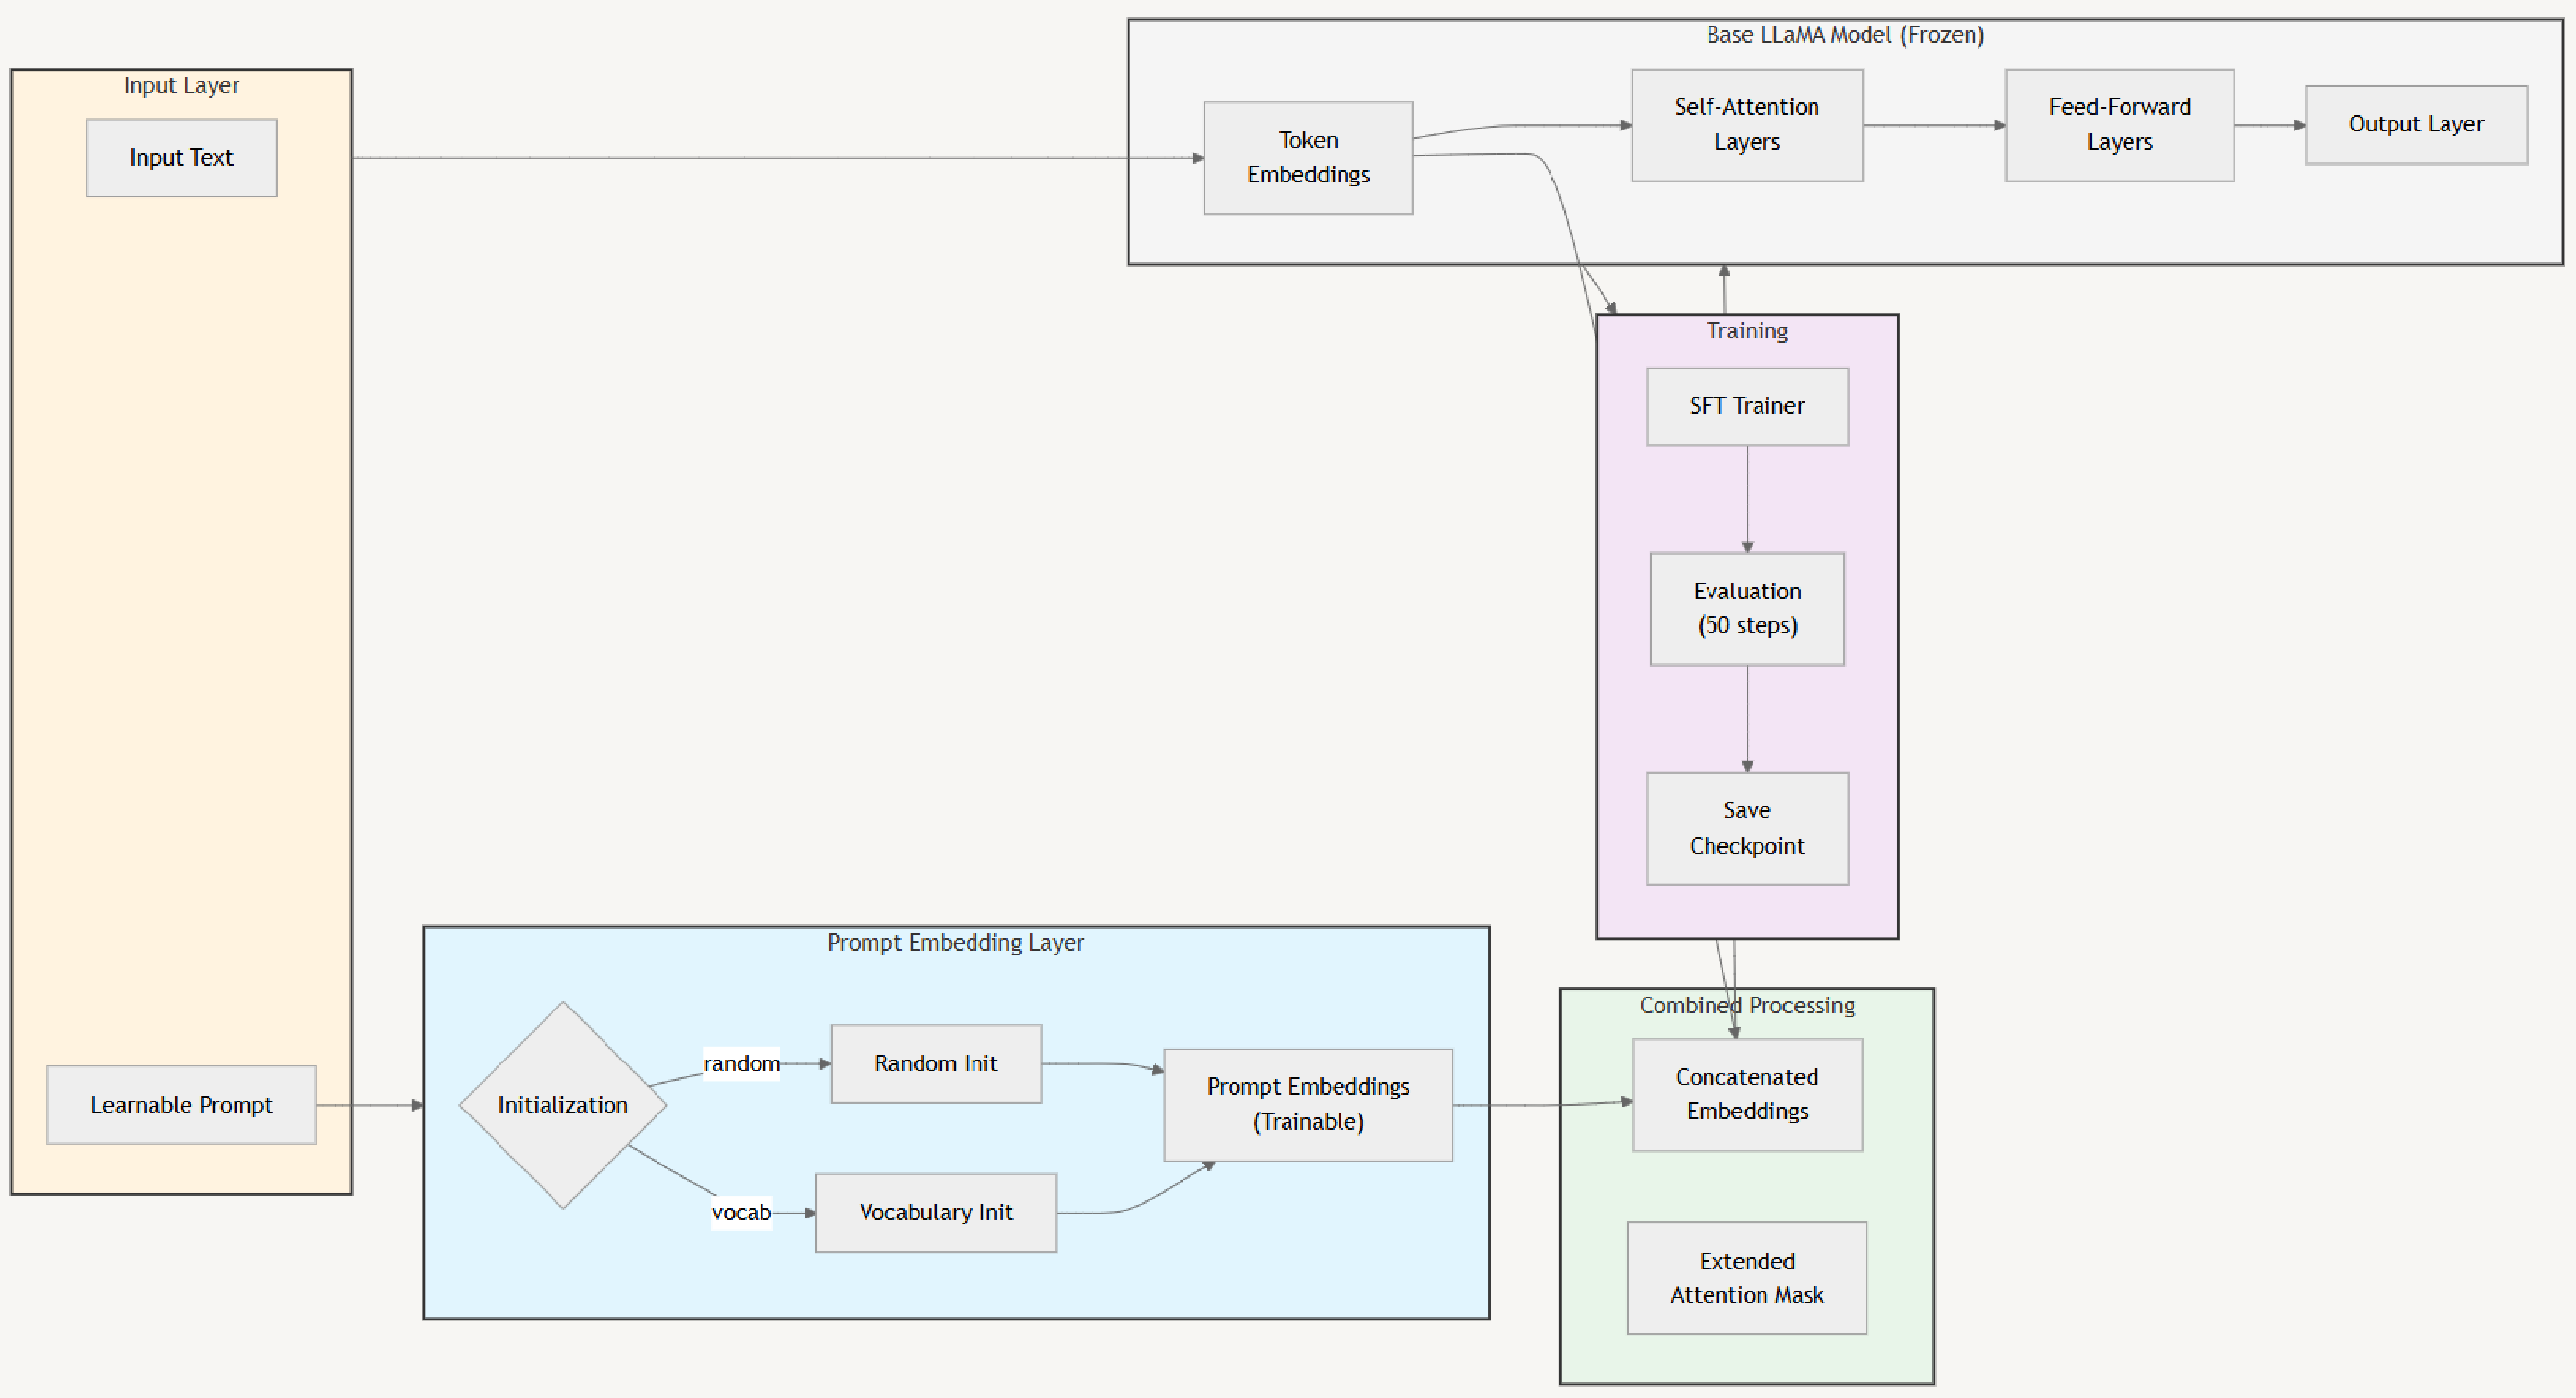
\includegraphics[width=0.8\textwidth]{./prompt_tuning_model}
    \caption{Prompt Tuning}
    \label{fig:prompt-tuning}
\end{figure*}



\section{Problem Definition \& Challenges}
\subsection{Challenges of the Project}
In this research, we focus on comparing different approaches to fine-tuning large language models for character-specific dialogue generation using the Harry Potter universe as our test case. As shown in Figure \ref{fig:lora-model} and Figure \ref{fig:prompt-tuning}, LoRA and Prompt Tuning represent fundamentally different approaches to model adaptation:

\begin{itemize}
    \item \textbf{Base Model with Quantization}: Using 4-bit quantization of Llama3-8b as our baseline
    \item \textbf{LoRA Fine-tuning}: As illustrated in Figure \ref{fig:lora-model}, this approach introduces trainable rank decomposition matrices alongside the frozen weights of the original model
    \item \textbf{Prompt Tuning}: Demonstrated in Figure \ref{fig:prompt-tuning}, this method prepends trainable continuous prompt embeddings to the input while keeping the model frozen
\end{itemize}

The primary challenges of this project include:
\begin{itemize}
    \item \textbf{Architecture-Specific Challenges:}
    \begin{itemize}
        \item \textbf{LoRA}: Determining optimal rank for the decomposition matrices while maintaining model stability
        \item \textbf{Prompt Tuning}: Finding the right balance between prompt length and training efficiency
        \item \textbf{Quantization}: Managing precision loss in 4-bit representation
    \end{itemize}
    \item \textbf{Training Dynamics:} Addressing the different convergence behaviors between LoRA's weight updates and Prompt Tuning's embedding optimization
    \item \textbf{Character Consistency:} Evaluating how each approach maintains character traits through their respective adaptation mechanisms
    \item \textbf{Resource Efficiency:} Comparing the memory and computational requirements of each method
\end{itemize}

\subsection{Main Purpose of the Project}
This project aims to systematically compare these architectural approaches, with particular attention to their unique characteristics as shown in our figures. Our key objectives include:

\begin{itemize}
\item \textbf{Architectural Comparison:}
    \begin{itemize}
        \item Analyze how LoRA's rank decomposition (Figure \ref{fig:lora-model}) affects dialogue generation quality
        \item Evaluate the effectiveness of Prompt Tuning's continuous embeddings (Figure \ref{fig:prompt-tuning})
        \item Compare both against the quantized baseline model
    \end{itemize}
    
\item \textbf{Implementation Analysis:}
    \begin{itemize}
        \item \textbf{For LoRA:}
        \begin{itemize}
            \item Optimize the low-rank update matrices shown in Figure \ref{fig:lora-model}
            \item Evaluate the impact of different rank values on performance
            \item Assess the balance between parameter efficiency and adaptation capability
        \end{itemize}
        \item \textbf{For Prompt Tuning:}
        \begin{itemize}
            \item Determine optimal prompt embedding dimensions as shown in Figure \ref{fig:prompt-tuning}
            \item Investigate prompt initialization strategies
            \item Analyze the relationship between prompt length and performance
        \end{itemize}
    \end{itemize}

\item \textbf{Comparative Evaluation:}
    \begin{itemize}
        \item Develop metrics that fairly compare these architecturally different approaches
        \item Assess each method's ability to capture character-specific dialogue patterns
        \item Compare computational and memory efficiency across approaches
        \item Analyze the trade-offs between model complexity and performance
    \end{itemize}
\end{itemize}

Through this structured comparison, we aim to provide insights into the relative strengths and weaknesses of each approach, particularly focusing on how their architectural differences (as shown in Figures \ref{fig:lora-model} and \ref{fig:prompt-tuning}) impact their effectiveness in character-specific dialogue generation.



\section{Related Works}
Recent advancements in character-based dialogue systems and large language models have created new opportunities for dynamic, personality-consistent conversation generation. This section examines key developments across commercial implementations and academic research that inform our approach.

\subsection{Commercial Implementation Analysis}
Character.ai represents a significant milestone in deployable character-based dialogue systems. Their implementation demonstrates the feasibility of maintaining consistent character personalities across multiple concurrent conversations while managing computational resources effectively. The platform's success in handling multiple simultaneous users provides valuable insights into scalable architecture design for character-based dialogue systems.

\subsection{Academic Research Foundations}
Recent academic work has established crucial frameworks for efficient model adaptation and personality-consistent dialogue generation:

\textbf{Parameter-Efficient Fine-tuning Approaches:}
\begin{itemize}
\item \textbf{Low-Rank Adaptation (LoRA)} \cite{hu2021} introduces an efficient approach to adapt large language models through low-rank decomposition matrices. By optimizing only these matrices instead of all model parameters, LoRA achieves remarkable efficiency while maintaining model performance. This method is particularly relevant for our goal of creating character-specific dialogue models with minimal computational overhead.

\item \textbf{Prompt Tuning} \cite{lester2021} demonstrates that by only optimizing continuous prompt embeddings, models can achieve performance comparable to full fine-tuning. Their work shows that as model size increases, the effectiveness of prompt tuning also increases, making it particularly suitable for our application with Llama3-8b.
\end{itemize}

\textbf{Character Alignment and Personality Modeling:}
\begin{itemize}
\item "Large Language Models Meet Harry Potter" \cite{chen2023} presents a comprehensive framework for character alignment in dialogue systems. The study introduces innovative techniques for maintaining personality consistency through carefully constructed attribute and relation matrices. Their methodology demonstrates how to effectively capture and maintain character-specific traits across extended dialogue sequences.
\item Character-LLM \cite{shao2023} builds upon this foundation by introducing a trainable agent specifically designed for role-playing scenarios. The system employs a novel architecture that combines transformer-based language modeling with personality embedding layers, achieving superior performance in maintaining character consistency across diverse conversation contexts.
\end{itemize}

\textbf{Multi-Character Dialogue Systems:}
\begin{itemize}
\item RoleLLM \cite{wang2023} provides a comprehensive benchmark for evaluating role-playing capabilities in large language models. The study introduces evaluation metrics specifically designed for assessing personality consistency and response appropriateness in character-based dialogue systems. Their findings suggest that attention-based architectures with character-specific prompt tuning achieve optimal performance in maintaining distinct personalities.
\item The Neeko framework \cite{yu2024} introduces dynamic LoRA (Low-Rank Adaptation) techniques for efficient multi-character role-playing. Their approach demonstrates how to switch between different character personalities with minimal computational overhead, achieving a 75\% reduction in parameter storage requirements while maintaining 95\% of the original performance metrics.
\end{itemize}

\textbf{Language-Specific Implementations:}
\begin{itemize}
\item CharacterGLM \cite{zhou2023} addresses the unique challenges of implementing character-based dialogue systems in Chinese language contexts. Their work provides valuable insights into handling language-specific nuances while maintaining character consistency, achieving state-of-the-art performance in Chinese character dialogue generation.
\end{itemize}



\section{Datasets}
In this project, \textbf{Harry-Potter-Dialogue-Dataset} introduced by \cite{chen2023} is used for fine-tuning LLM Models and standard for evaluating their purposes.

Harry Potter Dialogue is a dialogue dataset that integrates with scene, attributes and relations which are dynamically changed as the storyline goes on, which is deliberately designed to be used for researches on more human-like conversational systems in practice. For example, virtual assistant, NPC in games, etc. Moreover, HPD can both support dialogue generation and retrieval tasks.

It provides information about each character's 13 attributes such ad Gender, Age, Belongings, Hobby and Spells. Information about relations between characters is also given, which lets LLM to create more appropriate dialogues regarding to the context of the full story.



\section{Experimental Setup}

\subsection{Dataset Preprocessing and Augmentation}
Our implementation begins with comprehensive preprocessing of the Harry Potter Dialogue Dataset to optimize it for character-specific dialogue generation. The preprocessing pipeline consists of several key stages:

\textbf{Initial Data Restructuring:}
\begin{itemize}
\item Reorganized the complex multi-modal dataset into the Alpaca instruction format for more effective fine-tuning
\item Implemented progressive dialogue sequence processing to create training samples (see Algorithm \ref{alg:dialogue_processing})
\end{itemize}

\begin{algorithm}[tb]
   \caption{Dialogue Sequence Processing}
   \label{alg:dialogue_processing}
\begin{algorithmic}
   \STATE {\bfseries Input:} dialogue sequence $D = [d_1, d_2, ..., d_n]$
   \STATE {\bfseries Output:} training pairs $P$
   \STATE Initialize $P = []$
   \FOR{$i=2$ {\bfseries to} $n$}
      \STATE $context = [d_1, ..., d_{i-1}]$
      \STATE $target = d_i$
      \STATE Add $(context, target)$ to $P$
   \ENDFOR
   \RETURN $P$
\end{algorithmic}
\end{algorithm}

\textbf{Multi-stage Data Augmentation:}
\begin{itemize}
\item \textbf{Primary Augmentation:} Implemented dialogue-based sequence splitting and reconstruction
    \begin{itemize}
    \item Generated multiple training instances from each dialogue sequence
    \item Preserved contextual coherence while increasing dataset diversity
    \end{itemize}
\item \textbf{Secondary Augmentation:} Applied probabilistic content inclusion and semantic variation
    \begin{itemize}
    \item Selective inclusion of scene descriptions (p=0.8), character attributes (p=0.7), and relationship information (p=0.6)
    \item Utilized WordNet-based synonym replacement for scene descriptions
    \item Implemented random sampling of character attributes and relationships to create varied context combinations
    \end{itemize}
\end{itemize}

\subsection{Computing Infrastructure}
The experimental implementation utilized the following computational resources and frameworks:

\textbf{Hardware Configuration:}
\begin{itemize}
\item Google Colab Pro environment with T4 GPU acceleration
\item Optimized memory usage for handling large-scale model training
\end{itemize}

\textbf{Software Stack:}
\begin{itemize}
\item \textbf{Core Frameworks:}
    \begin{itemize}
    \item PyTorch for deep learning operations
    \item NLTK for natural language processing and data augmentation
    \item SFTTrainer for supervised fine-tuning
    \end{itemize}
\item \textbf{Optimization Tools:}
    \begin{itemize}
    \item Unsloth library for accelerated LoRA fine-tuning
    \item Custom data loading and processing utilities
    \end{itemize}
\end{itemize}

\subsection{Evaluation Metrics and Methodology}
We employ a comprehensive evaluation framework to assess the performance of our models across multiple dimensions:

\textbf{Automatic Metrics:}
\begin{itemize}
\item \textbf{BLEU} (Bilingual Evaluation Understudy): Measures the precision of generated responses against reference texts
\item \textbf{METEOR} (Metric for Evaluation of Translation with Explicit ORdering): Evaluates the quality of generated text by considering synonyms and paraphrases
\item \textbf{Perplexity}: Assesses the fluency and naturalness of generated dialogues
\item \textbf{SIMILE}: Measures semantic similarity between generated responses and ground truth using the Solar Embedding Model
\end{itemize}

\textbf{Training Parameters:}
\begin{itemize}
\item Learning rate: 3e-4 for LoRA, 1e-3 for Prompt Tuning
\item Batch size: 32
\item Training epochs: 10
\item LoRA rank: 8
\item Prompt tokens: 20
\item Weight decay: 0.01
\end{itemize}




\section{Results and Analysis}

Our experimental results reveal significant differences in dialogue generation quality across different model configurations, highlighting distinct strengths and limitations of each approach.

\begin{table}[t]
\caption{Performance Comparison of Model Configurations}
\label{tab:model-comparison}
\centering
\begin{tabular}{lcccc}
\toprule
Model Config & BLEU & MTR & PPL & SIM \\
\midrule
Base Llama & 1.11 & 10.64 & 113.47 & 0.59 \\
+ LoRA Fine-tuning & 21.91 & 26.75 & \textbf{26.46} & \textbf{0.95} \\
+ Prompt Tuning & \textbf{26.79} & \textbf{35.21} & 48.56 & 0.75 \\
\bottomrule
\end{tabular}
\smallskip
\begin{flushleft}
\small
MTR: METEOR, PPL: Perplexity, SIM: SIMILE \\
\end{flushleft}
\end{table}

\subsection{Model Performance Analysis}

\textbf{Base Model Performance:}
The base Llama3-8b model showed notably poor performance across all metrics (BLEU: 1.11, METEOR: 10.64, Perplexity: 113.47, SIMILE: 0.59). This indicates that the base model, despite its general language capabilities, fails to:
\begin{itemize}
\item Maintain consistent character voice
\item Generate contextually appropriate responses
\item Adhere to the established dialogue patterns in the Harry Potter universe
\end{itemize}

\textbf{Impact of LoRA Fine-tuning:}
The LoRA-enhanced model demonstrated substantial improvements, particularly in dialogue consistency and structural coherence:
\begin{itemize}
\item Achieved optimal perplexity (26.46) and semantic similarity (0.95) scores
\item Showed significant improvement in BLEU (21.91) and METEOR (26.75) scores compared to the base model
\item Exhibited strong character voice consistency and format adherence due to the fine-tuning process
\end{itemize}

\textbf{Prompt Tuning Results:}
The prompt-tuned model showed the highest performance in translation metrics while maintaining reasonable semantic coherence:
\begin{itemize}
\item Achieved the best BLEU (26.79) and METEOR (35.21) scores
\item Maintained good semantic similarity (0.75), though lower than LoRA
\item Showed higher perplexity (48.56) compared to LoRA, suggesting some trade-off in fluency
\end{itemize}

\subsection{Qualitative Analysis}

To provide deeper insights into the models' performance characteristics, we present example outputs from each model variant compared to ground truth responses in Table \ref{tab:qualitative}.

\begin{table*}[t]
\caption{Qualitative Comparison of Model Outputs Across Different Configurations}
\label{tab:qualitative}
\centering
\begin{tabular}{p{0.22\linewidth}|p{0.78\linewidth}}
\toprule
\textbf{Context} & \textit{Previous Dialogue:} \\
& "D'you think he'll be all right?" \\
& "Course he will. Madam Pomfrey can mend cuts in about a second." \\
& "That was a really bad thing to happen in Hagrid's first class, though, wasn't it? Trust Malfoy to mess things up for him..." \\ 
\midrule
\textbf{Ground Truth} & {\color{black} "Yeah it must be. Malfoy will even ask the school to fire Hagrid."} \\
\midrule
\textbf{Base Llama} & {\color{red} "I don't know what you're talking about. Let's discuss the Quidditch match instead."} \\
\midrule
\textbf{LoRA Fine-tuning} & {\color{green} "Yeah, and knowing Malfoy, he'll probably run straight {\color{red}to his father} to get Hagrid sacked."} \\
\midrule
\textbf{Prompt Tuning} & {\color{green} "Yeah, it must be terrible. I bet Malfoy will try to get Hagrid fired over this."} \\
\bottomrule
\end{tabular}
\end{table*}

The example demonstrates how different approaches affect response generation:

\begin{itemize}
    \item The \textbf{Base Model} completely fails to maintain context, generating an irrelevant response that ignores both the situation and character relationships. This aligns with its poor performance metrics across all categories.
    
    \item The \textbf{LoRA Fine-tuning} model captures the essence of the situation and character relationships well, particularly in maintaining the narrative context about Malfoy's character and his likely actions. The mention of "his father" shows strong understanding of character backgrounds, though the specific phrasing differs from the ground truth.
    
    \item The \textbf{Prompt Tuning} model generates a response most similar to the ground truth, accurately capturing both the situation and the likely consequences. This aligns with its superior BLEU and METEOR scores, though the slight differences in phrasing reflect the occasional hallucinations observed in our broader analysis.
\end{itemize}


\subsection{Comparative Discussion}

Our analysis reveals several key insights about the effectiveness of different approaches:

1. \textbf{Fine-tuning Necessity:} The poor performance of the base model demonstrates that raw LLM capabilities are insufficient for character-specific dialogue generation, necessitating some form of adaptation.

2. \textbf{Architecture Influence:} 
\begin{itemize}
\item LoRA's superior performance in perplexity and SIMILE suggests its effectiveness in maintaining structural consistency and character voice
\item Prompt tuning's higher BLEU and METEOR scores indicate better capture of character-specific language patterns
\end{itemize}

3. \textbf{Trade-off Patterns:} Each approach shows distinct trade-offs:
\begin{itemize}
\item LoRA prioritizes consistency and fluency over exact matching with reference responses
\item Prompt tuning achieves better reference matching but with slightly higher risk of hallucination
\end{itemize}

These results suggest that the choice between LoRA and prompt tuning may depend on specific application requirements, with LoRA being preferable for maintaining consistent character voice and dialogue structure, while prompt tuning might be better suited for applications prioritizing linguistic accuracy and character trait expression.



\section{Limitations and Future Work}

While our study provides valuable insights into parameter-efficient fine-tuning methods for character dialogue generation, several limitations should be acknowledged:

\subsection{Technical Limitations}

\textbf{Combined Optimization Approaches:}
\begin{itemize}
\item Due to time constraints, we were unable to explore the potential synergistic effects of combining LoRA and Prompt Tuning approaches
\item The interaction between these methods and their potential complementary benefits remains an open question for future research
\end{itemize}

\textbf{Model Diversity:}
\begin{itemize}
\item Our study focused solely on the Llama3-8b architecture
\item Comparative analysis with other state-of-the-art models such as Mistral and Gemma could provide valuable insights into the generalizability of our findings
\item Different model architectures might exhibit varying degrees of effectiveness with LoRA and Prompt Tuning techniques
\end{itemize}

\subsection{Methodological Limitations}

\textbf{Character Personalization:}
\begin{itemize}
\item The current implementation lacks character-specific fine-tuning based on individual personality traits and dialogue patterns
\item We did not fully utilize the rich character information available in the dataset for personalized model optimization
\item Future work could explore methods for extracting and incorporating character-specific features into the fine-tuning process
\end{itemize}

\textbf{Evaluation Methodology:}
\begin{itemize}
\item While we proposed comprehensive evaluation metrics including Semantic Role Labeling (SRL) and LIWC-based personality consistency analysis, time constraints prevented their implementation
\item The lack of these sophisticated evaluation methods limits our ability to fully assess the models' capability in maintaining character consistency and relationship dynamics
\item A more rigorous evaluation framework incorporating these metrics would provide deeper insights into model performance
\end{itemize}

\subsection{Future Research Directions}

Based on these limitations, we propose several promising directions for future research:

\begin{itemize}
\item Implementation of combined LoRA and Prompt Tuning approaches to explore potential performance improvements
\item Comprehensive comparative study across different model architectures (Llama3, Mistral, Gemma) to identify optimal base models for character dialogue generation
\item Development of character-specific fine-tuning strategies that leverage individual personality traits and relationship dynamics
\item Implementation of the proposed advanced evaluation metrics to better assess character consistency and dialogue quality
\end{itemize}

These limitations and future research directions highlight the significant potential for further advancement in character-based dialogue generation systems.



\bibliography{main}
\bibliographystyle{icml2019}

\clearpage

\end{document}